\begin{thm} Let $A\in \{0,1,-1\}^{m\times m}$, where each column has at most one $-1$ and at most one $1$ entry. Then $A$ is totally unimodular.
\end{thm}

\begin{pr} Let $N$ be a $k\times k$ submatrix of $A$. We do induction on $k$. For $k=1$ it's trivial.

Remember, determinants can be computed like this

\[\det A = \sum_{i=1}^n a_{ij} \cdot (-1)^{i+j} \det A_{ij} = \sum_{j=1}^n a_{ij} \cdot (-1)^{i+j} \det A_{ij}\]

There are two cases

\begin{itemize}
\item If $N$ has a column with at most one non-zero entry. We can just expand on that column to reduce the determinant of $N$ to the determinant of one $k-1\times k-1$ submatrix $N'$.

\item If all columns of $N$ have 2 non-zero entries (more are impossible by definition of $A$), the sum of all rows is $0$ so $N$ is singular and the determinant is $0$
\end{itemize}
\qed \end{pr}

A nice corollary from this theorem is the fact that the node-edge incidence matrix (rows=vertices, columns=edges, $1$ if edge is at vertex) of any digraph is TU.

\chapter{Solving Integer Programs}
\section{Cutting Planes and Cutting Plane Algorithms}
In most cases the ployhedron we describe with our integer linear program is not nicely integral.

A cutting plane algorithm tries to cut off parts of the polyhedron that are not in the integer hull of the polyhedron.

The idea here is that it's easy to find the integer hull of a halfplane. 

\[\trans a x \leq b \quad \Rightarrow \quad \trans a x \leq \lfloor b \rfloor\]

where the inequality is scaled s.t. $a$ is integral and $\gcd(a)=1$. Rounding down the right hand side shifts the hyperplane such that it intersects with the closest feasible integer point. Of course we'd need to round up in case of a $\geq$.

\begin{figure}[hbt]
\begin{center}
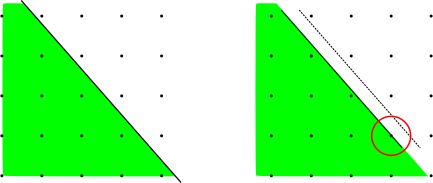
\includegraphics{./images/roundDownCuttingPlane}
\end{center}
\caption{The Integer Hull of a Halfplane}
\end{figure}

We could to this transformation for every valid constraint for the polyhedron and obtain the integer hull. However there are quite a few such cuts and we'd need to iterate the process because the new inequalities change the set of valid constraints.

Instead we just try to cut off things around the optimal solution until it becomes integral. That means we don't have to care about the other parts of the polyhedron and hopefully speeds up the process.

To find the right cutting planes we first solve the linear program relaxation to get some $x^*$. Then we find some hyperplane that cuts off $x^*$ without touching the integer hull, i.e. it is valid for $P_I$, and add it to our LP.

\begin{lstlisting}
repeat
	$x^*$ = Solve LP $\max \{cx|x\in P\}$
	if $x^*$ is integral return $x^*$
	$H$ = halfspace that separates $x^*$ from $P_I$
	$P=P\cap H$
\end{lstlisting}

Of course we don't know how to find the cutting plane that cuts off $x^*$, or even how to check if a given inequality is valid for $P_I$. It's also not clear if this algorithm always terminates and if it terminates how long it takes. Note though that we know that the halfplane must exist because of Farkas' Lemma.

\subsection{Cutting plane proofs}

There are many different ways to find cutting planes. In the following we will deal with Gomory-Chv\'{a}tal cuts.

We want to prove that some inequality $\trans cx\leq \delta$ is valid for all integral solutions of $Ax\leq b$. In particular we want to derive a series of cuts that are valid for all integral points but cut off the optimal solution $x^*$. We will refer to a series of cuts as a cutting plane proof.

\begin{Ex}
Let the system be

\[\begin{pmatrix}
2 & 3\\
2 & -2 \\
-6 & -2\\
-2 & -6\\
-6 & 8
\end{pmatrix}\cdot x \leq \begin{pmatrix} 27\\7\\-9\\-11\\21\end{pmatrix}\]

We want to prove that $x_2\leq 5$ is a valid inequality for the integer hull of this polyhedron. There is a fractional vector $(9/2,6)$ with $x_2=6$ though, so we want to find cuts that remove it.

We look at linear combinations of the rows. For example we see by scaling rows 5:

\[-3x_1+4x_2 \leq \frac{21}{2}\]

This means we can round down $21/2$ to $10$ because $x_1,x_2$ are integral. From adding two times that new inequality to three times the first one we get

\[17x_2 \leq 101 \quad \Rightarrow \quad x_2 \leq \left\lfloor \frac{101}{17}\right\rfloor = 5\]
\end{Ex}

In general we want to find inequalities of the form

\[\trans y A x \leq \left\lfloor \trans y b \right \rfloor,\quad y\geq 0, \trans y A \text{ integral}\]

These inequalities are called Gomory-Chv\'{a}tal cutting planes.

\begin{Def} Let $Ax\leq b$ system of $m$ linear inequalities and $\trans cx\leq \delta$ an inequality. A sequence of linear inequalities $c_1x\leq \delta_1, c_2x\leq \delta_2,\ldots, c_mx\leq \delta_m$ is called a \emph{cuting plane proof} of $\trans c x\leq \delta$ from $Ax\leq b$ if
\begin{itemize}
\item $c_1,\ldots c_m$ are integral
\item $c_m=c$ and $\delta_m=\delta$
\item $\forall i\in [1,m]: c_ix\leq \delta_i'$ is a nonnegative linear combination of inequalities from the system

\[Ax\leq b, c_1x\leq \delta_1,\ldots,c_{i-1}x\leq \delta_{i-1}\]

and $\delta_i=\lfloor \delta_i'\rfloor$.
\end{itemize}
\end{Def}

\begin{thm}[Existence]\label{thm:existsCuttingProof} Let $P=\{x\in \R^n | Ax\leq b\}$ be bounded and non-empty

\begin{enumerate}
\item if $P_I\neq \emptyset$ and some inequality $\trans c x\leq \delta$ with integral $c$ is valid, then there is a cutting plane proof
\item if $P_I=\emptyset$ then there is a cutting plane proof of 
\[0x\leq -1\]
\end{enumerate}
\end{thm}

Theorem \ref{thm:existsCuttingProof} gives us an "easy" way to check if a polyhedron has no integer vertices at all. This is in spirit similar to the result we had from the Farkas lemma for arbitrary constraint systems.

\begin{thm}[Finite Length] Let $Ax\leq s$ be a rational system of linear inequalities with at least one integral solution If $\trans cx\leq \delta$ is valid for integral $c$, then $\trans cx\leq \delta$ has a cutting plane proof of finite length.
\end{thm}

While looking for Gomory-Chv\'{a}tal cuts we usually use the cuts we already added to form new cuts. If we don't do that but instead add all cuts that we can form without taking into account the new constraints we form the Chv\'{a}tal closure of the polyhedron. It may seem that computing the Chv\'atal closure is impossible, because there are infinitely many such cuts.

However the following definition fully captures the Chv\'atal closure:

\begin{Def} Let $P=\{x|Ax\leq b\}$ be a rational polyhedron. Adding all Gomory-Chv\'{a}tal cuts $\trans yAx\leq \lfloor \trans y b\rfloor$ for $0\leq y < 1$ and $\trans y A$ integral, yields the \emph{Chv\'{a}tal Closure}
\end{Def}

To show why the definition captures the intuition of the closure we'll prove the following theorem.

\begin{thm} The Chv\'{a}tal Closure is a rational polyhedron that is equal to the set of points $P'$ that satisfies all valid Gomory-Chv\'atal cuts.\end{thm}

\begin{pr} Let $P=\{x|Ax\leq b\}$. Since we assume it is rational we can scale that up until everything is integral. We want to prove that $P'$, the set of all points that satisfy all Chv\'atal cuts, is defined by

\[\left({A}\atop{\trans y A}\right) x \leq \left({b}\atop {\lfloor \trans y b\rfloor}\right)\]

for $y$ with $0\leq y < 1$ and $\trans y A$ is integral. To do so we'll show that all possible cuts can be written as a linear combination of the constraints in $A$ plus one of the constraints we add.

So take some cut $\trans w x \leq \lfloor t\rfloor$ that has been derived from $A$ with some positive vector $\bar y$. Let $\bar y'= \bar y - \lfloor \bar y\rfloor$ be the fractional parts of that vector and consider $w'=\trans {\bar y'}A$. We can write $w'=w-\trans{\lfloor \bar y \rfloor}A$, so we know that $w'$ must be integral since $w$ is integral by definition of a Gomory-Chv\'atal cut and the product $\trans{\lfloor \bar y \rfloor}A$ only contains integral numbers. By a similar argument we can see that $t' = \trans{\bar y'}b$ differs from $t$ by an integral amount.

So we have the constraint $\trans {w'}x\leq \lfloor t'\rfloor$ that we must have added because $w'$ is integral and a combination of the rows of $A$ and the constraint $\trans{\lfloor \bar y \rfloor} Ax\leq \trans{\lfloor \bar y\rfloor} b$ which is a linear combination of the rows of $A$. If we add them both up we get back the constraint $\trans w x\leq t$, which concludes the proof.
\qed \end{pr}

Hence there is a finite description of the Chv\'atal closure for a polyhedron.